\documentclass[12pt]{report}
\usepackage[utf8]{inputenc}
\usepackage[russian]{babel}
%\usepackage[14pt]{extsizes}
\usepackage{listings}
\usepackage{graphicx}
\usepackage{amsmath,amsfonts,amssymb,amsthm,mathtools} 
\usepackage{pgfplots}
\usepackage{filecontents}
\usepackage{float}
\usepackage{indentfirst}
\usepackage{eucal}
\usepackage{enumitem}
\frenchspacing

\usepackage{indentfirst} % Красная строка


\usetikzlibrary{datavisualization}
\usetikzlibrary{datavisualization.formats.functions}

\usepackage{amsmath}




% Для листинга кода:
\lstset{ %
language=haskell,                 % выбор языка для подсветки (здесь это С)
basicstyle=\small\sffamily, % размер и начертание шрифта для подсветки кода
numbers=left,               % где поставить нумерацию строк (слева\справа)
numberstyle=\tiny,           % размер шрифта для номеров строк
stepnumber=1,                   % размер шага между двумя номерами строк
numbersep=5pt,                % как далеко отстоят номера строк от подсвечиваемого кода
showspaces=false,            % показывать или нет пробелы специальными отступами
showstringspaces=false,      % показывать или нет пробелы в строках
showtabs=false,             % показывать или нет табуляцию в строках
frame=single,              % рисовать рамку вокруг кода
tabsize=2,                 % размер табуляции по умолчанию равен 2 пробелам
captionpos=t,              % позиция заголовка вверху [t] или внизу [b] 
breaklines=true,           % автоматически переносить строки (да\нет)
breakatwhitespace=false, % переносить строки только если есть пробел
escapeinside={\#*}{*)}   % если нужно добавить комментарии в коде
}

\usepackage[left=2cm,right=2cm, top=2cm,bottom=2cm,bindingoffset=0cm]{geometry}
% Для измененных титулов глав:
\usepackage{titlesec, blindtext, color} % подключаем нужные пакеты
\definecolor{gray75}{gray}{0.75} % определяем цвет
\newcommand{\hsp}{\hspace{20pt}} % длина линии в 20pt
% titleformat определяет стиль
\titleformat{\chapter}[hang]{\Huge\bfseries}{\thechapter\hsp\textcolor{gray75}{|}\hsp}{0pt}{\Huge\bfseries}


% plot
\usepackage{pgfplots}
\usepackage{filecontents}
\usetikzlibrary{datavisualization}
\usetikzlibrary{datavisualization.formats.functions}

\begin{document}
%\def\chaptername{} % убирает "Глава"
\thispagestyle{empty}
\begin{titlepage}
	\noindent \begin{minipage}{0.15\textwidth}
	
\includegraphics[width=\linewidth]{img/b_logo}
	\end{minipage}
	\noindent\begin{minipage}{0.9\textwidth}\centering
		\textbf{Министерство науки и высшего образования Российской Федерации}\\
		\textbf{Федеральное государственное бюджетное образовательное учреждение высшего образования}\\
		\textbf{~~~«Московский государственный технический университет имени Н.Э.~Баумана}\\
		\textbf{(национальный исследовательский университет)»}\\
		\textbf{(МГТУ им. Н.Э.~Баумана)}
	\end{minipage}
	
	\noindent\rule{18cm}{3pt}
	\newline\newline
	\noindent ФАКУЛЬТЕТ $\underline{\text{«Информатика и системы управления»}}$ \newline\newline
	\noindent КАФЕДРА $\underline{\text{«Программное обеспечение ЭВМ и информационные технологии»}}$\newline\newline\newline\newline\newline
	
	
	\begin{center}
		\noindent\begin{minipage}{1.3\textwidth}\centering
			\Large\textbf{  Отчет по лабораторной работе №4}\newline
			\textbf{по дисциплине "Операционные системы"}\newline\newline
		\end{minipage}
	\end{center}
	
	\noindent\textbf{Тема} $\underline{\text{Процессы. Системные вызовы fork() и exec()}}$\newline\newline
	\noindent\textbf{Студент} $\underline{\text{Зайцева А. А.~~~~~~~~~~~~~~~~~~~~~~~~~~~~~~~~~~~~~~}}$\newline\newline
	\noindent\textbf{Группа} $\underline{\text{ИУ7-52Б~~~~~~~~~~~~~~~~~~~~~~~~~~~~~~~~~~~~~~~~~~~~~~}}$\newline\newline
	\noindent\textbf{Оценка (баллы)} $\underline{\text{~~~~~~~~~~~~~~~~~~~~~~~~~~~~~~~~~~~~~~~~~~~~~}}$\newline\newline
	\noindent\textbf{Преподаватели} $\underline{\text{Рязанова Н.Ю.~~~~~~~~~~~~~~~~~~~~~~~~~~}}$\newline\newline\newline
	
	\begin{center}
		\vfill
		Москва~---~\the\year
		~г.
	\end{center}
\end{titlepage}

\newpage

\section*{Задание №1}


Процессы-сироты. В программе создаются не менее двух потомков. В потомках вызывается sleep(). Чтобы предок гарантированно завершился раньше своих помков. Продемонстрировать с помощью соответствующего вывода информацию об идентификаторах процессов и их группе.

\begin{lstlisting}[label=some-code,caption=Код программы к заданию №1,language=C]
#include <stdio.h>
#include <unistd.h>
#include <stdlib.h>

#define RET_OK 0
#define RET_ERR_FORK 1

#define FORK_OK 0
#define FORK_ERR -1

#define INTERVAL 1

int main()
{
	pid_t childpid1, childpid2;
	if ((childpid1 = fork()) == FORK_ERR)
	{
		perror("Can't fork first child process.\n");
		return RET_ERR_FORK;
	}
	else if (childpid1 == FORK_OK)
	{
		printf("First child process: pid = %d, ppid = %d, pgrp = %d\n", 
		getpid(), getppid(), getpgrp());
		
		sleep(INTERVAL);
		printf("First child process (has become an orphan): pid = %d, ppid = %d, pgrp = %d\n", 
		getpid(), getppid(), getpgrp());
		
		printf("First child process is dead now\n");
		
		exit(RET_OK);
	}
	
	
	if ((childpid2 = fork()) == FORK_ERR)
	{
		perror("Can't fork second child process.\n");
		return RET_ERR_FORK;
	}
	else if (childpid2 == FORK_OK)
	{
		printf("Second child process: pid = %d, ppid = %d, pgrp = %d\n", 
		getpid(), getppid(), getpgrp());
		
		sleep(INTERVAL);
		printf("Second child process (has become an orphan): pid = %d, ppid = %d, pgrp = %d\n", 
		getpid(), getppid(), getpgrp());
		
		printf("Second child process is dead now\n");
		exit(RET_OK);
	}
	
	printf("Parent process: pid = %d, pgrp = %d, childpid1 = %d, childpid2 = %d\n", 
	getpid(), getpgrp(), childpid1, childpid2);
	printf("Parent process is dead now\n");
	return RET_OK;
	
}
\end{lstlisting}

\begin{figure}[H]

	\centering

	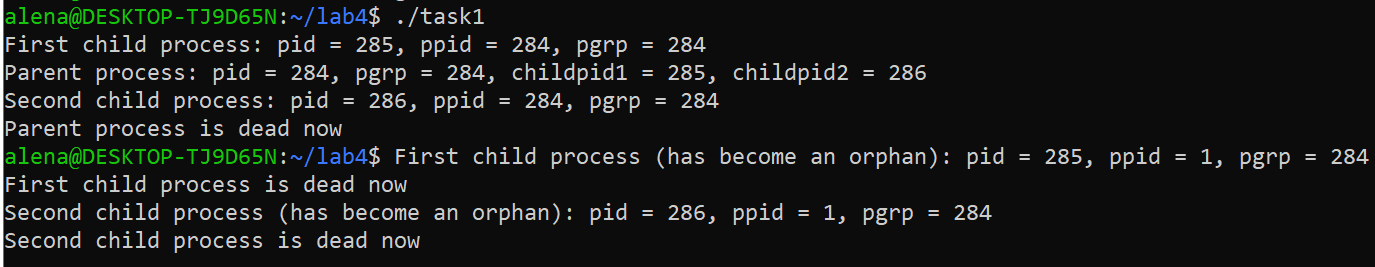
\includegraphics[width=\linewidth]{img/task01.png}
	\caption{Демонстрация работы программы (задание №1).}

	\label{fig:task01}

\end{figure}

\section*{Задание №2}

Предок ждет завершения своих потомком, используя системный вызов wait(). Вывод соответствующих сообщений на экран.

\begin{lstlisting}[label=some-code,caption=Код программы к заданию №2,language=C]
#include <stdio.h>
#include <unistd.h>
#include <stdlib.h>
#include <sys/wait.h>

#define RET_OK 0
#define RET_ERR_FORK 1

#define FORK_OK 0
#define FORK_ERR -1

#define INTERVAL 1

int main()
{
	pid_t childpid1, childpid2, childpid;
	if ((childpid1 = fork()) == FORK_ERR)
	{
		perror("Can't fork first child process.\n");
		return RET_ERR_FORK;
	}
	else if (childpid1 == FORK_OK)
	{
		printf("First child process: pid = %d, ppid = %d, pgrp = %d\n", 
		getpid(), getppid(), getpgrp());
		
		exit(RET_OK);
	}
	
	if ((childpid2 = fork()) == FORK_ERR)
	{
		perror("Can't fork second child process.\n");
		return RET_ERR_FORK;
	}
	else if (childpid2 == FORK_OK)
	{
		printf("Second child process: pid = %d, ppid = %d, pgrp = %d\n", 
		getpid(), getppid(), getpgrp());
		
		exit(RET_OK);
	}
	
	sleep(INTERVAL);
	printf("Parent process: pid = %d, pgrp = %d, childpid1 = %d, childpid2 = %d\n", 
	getpid(), getpgrp(), childpid1, childpid2);
	
	int ch_status;
	for (int i = 0; i < 2; i++)
	{
		childpid = wait(&ch_status);
		printf("Child with pid = %d has finished with status %d\n", childpid, ch_status);
		
		if (WIFEXITED(ch_status))
		printf("Child exited normally with exit code %d\n", WEXITSTATUS(ch_status));
		else if (WIFSIGNALED(ch_status))
		printf("Child process ended with a non-intercepted signal number %d\n", WTERMSIG(ch_status));
		else if (WIFSTOPPED(ch_status))
		printf("Child process was stopped by a signal %d\n", WSTOPSIG(ch_status));
	}
	
	printf("Parent process is dead now\n");
	return RET_OK;
}
\end{lstlisting}

\begin{figure}[H]

	\centering

	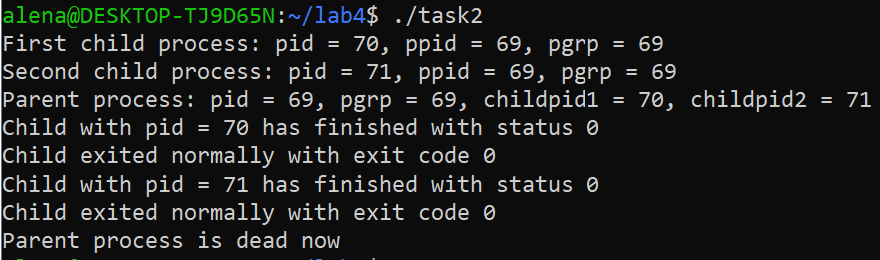
\includegraphics[width=\linewidth]{img/task02.png}
	\caption{Демонстрация работы программы (задание №2).}

	\label{fig:task02}

\end{figure}

\section*{Задание №3}

Потомки переходят на выполнение других программ. Предок ждет завершения своих потомков. Вывод соответствующих сообщений на экран.


\begin{lstlisting}[label=some-code,caption=Код программы к заданию №3,language=C]
#include <stdio.h>
#include <unistd.h>
#include <stdlib.h>
#include <sys/wait.h>

#define RET_OK 0
#define RET_ERR_FORK 1
#define RET_CANT_EXECLP 2

#define FORK_OK 0
#define FORK_ERR -1

#define INTERVAL 1

int main()
{
	pid_t childpid1, childpid2, childpid;
	if ((childpid1 = fork()) == FORK_ERR)
	{
		perror("Can't fork first child process.\n");
		return RET_ERR_FORK;
	}
	else if (childpid1 == FORK_OK)
	{
		printf("First child process: pid = %d, ppid = %d, pgrp = %d\n", 
		getpid(), getppid(), getpgrp());
		if (execlp("echo" , "echo" , "This is echo command from first child", NULL) < 0)
		{
			perror("Can't execlp from first child.\n");
			exit(RET_CANT_EXECLP);
		}
		exit(RET_OK);
	}
	
	if ((childpid2 = fork()) == FORK_ERR)
	{
		perror("Can't fork second child process.\n");
		return RET_ERR_FORK;
	}
	else if (childpid2 == FORK_OK)
	{
		printf("Second child process: pid = %d, ppid = %d, pgrp = %d\n", 
		getpid(), getppid(), getpgrp());
		if (execlp("cat", "cat", "for_cat.txt", NULL) < 0)
		{
			perror("Can't execlp from second child.\n");
			exit(RET_CANT_EXECLP);
		}
		
		exit(RET_OK);
	}
	
	sleep(INTERVAL);
	printf("Parent process: pid = %d, pgrp = %d, childpid1 = %d, childpid2 = %d\n", 
	getpid(), getpgrp(), childpid1, childpid2);
	
	int ch_status;
	for (int i = 0; i < 2; i++)
	{
		childpid = wait(&ch_status);
		printf("Child with pid = %d has finished with status %d\n", childpid, ch_status);
		
		if (WIFEXITED(ch_status))
		printf("Child exited normally with exit code %d\n", WEXITSTATUS(ch_status));
		else if (WIFSIGNALED(ch_status))
		printf("Child process ended with a non-intercepted signal number %d\n", WTERMSIG(ch_status));
		else if (WIFSTOPPED(ch_status))
		printf("Child process was stopped by a signal %d\n", WSTOPSIG(ch_status));
	}
	
	printf("Parent process is dead now\n");
	return RET_OK;
}
\end{lstlisting}

\begin{figure}[H]

	\centering

	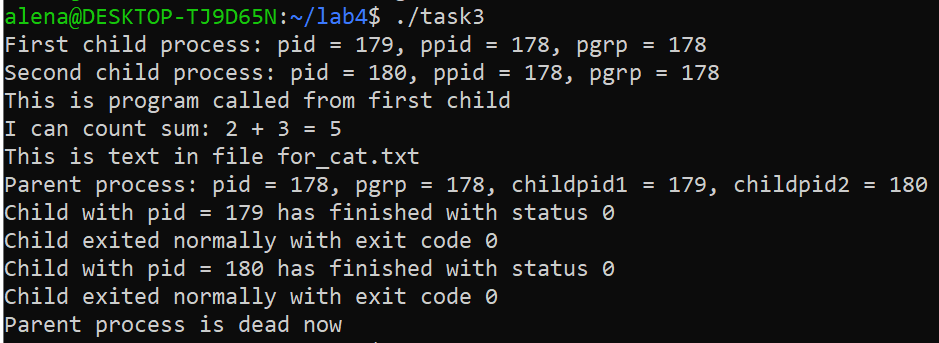
\includegraphics[width=\linewidth]{img/task03.png}
	\caption{Демонстрация работы программы (задание №3).}

	\label{fig:task03}

\end{figure}

\section*{Задание №4}

Предок и потомки обмениваются сообщениями через неименованный программный канал. Предок ждет завершения своих потомков. Вывод соответствующих сообщений на экран.

\begin{lstlisting}[label=some-code,caption=Код программы к заданию №4,language=C]
#include <stdio.h>
#include <unistd.h>
#include <stdlib.h>
#include <sys/wait.h>
#include <string.h>

#define RET_OK 0
#define RET_ERR_FORK 1
#define RET_ERR_PIPE 2

#define FORK_OK 0
#define FORK_ERR -1

#define INTERVAL 1
#define N_CHILDS 2
#define MSG1 "This is message from 1 child\n"
#define MSG2 "This is message from 2 child\n"
#define LEN12 30

int main()
{
	pid_t childpid1, childpid2, childpid;
	int fd[2];
	
	if (pipe(fd) == -1)
	{
		perror("Can't pipe\n");
		return RET_ERR_PIPE;
	}
	
	
	if ((childpid1 = fork()) == FORK_ERR)
	{
		perror("Can't fork first child process.\n");
		return RET_ERR_FORK;
	}
	else if (childpid1 == FORK_OK)
	{
		printf("First child process: pid = %d, ppid = %d, pgrp = %d\n", 
		getpid(), getppid(), getpgrp());
		
		close(fd[0]);
		write(fd[1], MSG1, strlen(MSG1) + 1);
		printf("Message from first child was sent\n"); 
		
		exit(RET_OK);
	}
	
	if ((childpid2 = fork()) == FORK_ERR)
	{
		perror("Can't fork second child process.\n");
		return RET_ERR_FORK;
	}
	else if (childpid2 == FORK_OK)
	{
		printf("Second child process: pid = %d, ppid = %d, pgrp = %d\n", 
		getpid(), getppid(), getpgrp());
		
		close(fd[0]);
		write(fd[1], MSG2, strlen(MSG2) + 1);
		printf("Message from second child was sent\n"); 
		
		exit(RET_OK);
	}
	
	sleep(INTERVAL);
	printf("Parent process: pid = %d, pgrp = %d, childpid1 = %d, childpid2 = %d\n", 
	getpid(), getpgrp(), childpid1, childpid2);
	
	int ch_status;
	for (int i = 0; i < N_CHILDS; i++)
	{
		childpid = wait(&ch_status);
		printf("Child with pid = %d has finished with status %d\n", childpid, ch_status);
		
		if (WIFEXITED(ch_status))
		printf("Child exited normally with exit code %d\n", WEXITSTATUS(ch_status));
		else if (WIFSIGNALED(ch_status))
		printf("Child process ended with a non-intercepted signal number %d\n", WTERMSIG(ch_status));
		else if (WIFSTOPPED(ch_status))
		printf("Child process was stopped by a signal %d\n", WSTOPSIG(ch_status));
	}
	
	char message[LEN12] = { 0 };
	
	printf("Reading messages from children.\n");
	close(fd[1]);
	
	for (int i = 0; i < N_CHILDS; i++)
	{
		
		if (read(fd[0], message, LEN12) < 0)
		printf("No messages from child %d.\n", i+1);
		else
		printf("Message from child %d:\n%s", i+1, message);
	}
	
	printf("Parent process is dead now\n");
	return RET_OK;
}
\end{lstlisting}

\begin{figure}[H]

	\centering

	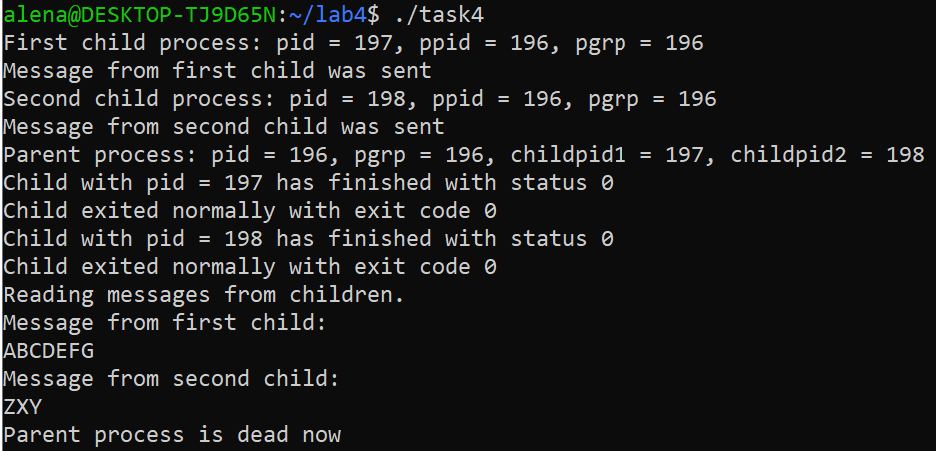
\includegraphics[width=\linewidth]{img/task04.png}
	\caption{Демонстрация работы программы (задание №4).}

	\label{fig:task04}

\end{figure}

\section*{Задание №5}

Предок и потомки обмениваются сообщениями через неименованный программный канал. С помощью сигнала меняется ход выполнения программы. Предок ждет завершения своих потомков. Вывод соответствующих сообщений на экран.

\begin{lstlisting}[label=some-code,caption=Код программы к заданию №5,language=C]
#include <stdio.h>
#include <unistd.h>
#include <stdlib.h>
#include <sys/wait.h>
#include <string.h>
#include <signal.h>

#define RET_OK 0
#define RET_ERR_FORK 1
#define RET_ERR_PIPE 2

#define FORK_OK 0
#define FORK_ERR -1

#define BIG_INTERVAL 1000
#define SMALL_INTERVAL 800
#define N_CHILDS 2
#define MSG1 "This is message from 1 child\n"
#define MSG2 "This is message from 2 child\n"
#define LEN12 30

void child1_exit(int sig_numb) 
{
	printf("First child exits\n");
	exit(RET_OK);
}

void child2_exit(int sig_numb) 
{
	printf("Second child exits\n");
	exit(RET_OK);
}


int main()
{
	pid_t childpid1, childpid2, childpid;
	int fd[2];
	
	signal(SIGUSR1, child1_exit);
	signal(SIGUSR2, child2_exit);
	
	if (pipe(fd) == -1)
	{
		perror("Can't pipe\n");
		return RET_ERR_PIPE;
	}
	
	
	if ((childpid1 = fork()) == FORK_ERR)
	{
		perror("Can't fork first child process.\n");
		return RET_ERR_FORK;
	}
	else if (childpid1 == FORK_OK)
	{
		printf("First child process: pid = %d, ppid = %d, pgrp = %d\n", 
		getpid(), getppid(), getpgrp());
		
		close(fd[0]);
		write(fd[1], MSG1, strlen(MSG1) + 1);
		printf("Message from first child was sent\n"); 
		
		while (1)
		{
			printf("First child in infinite loop\n"); 
			usleep(SMALL_INTERVAL);
		}
	}
	
	if ((childpid2 = fork()) == FORK_ERR)
	{
		perror("Can't fork second child process.\n");
		return RET_ERR_FORK;
	}
	else if (childpid2 == FORK_OK)
	{
		printf("Second child process: pid = %d, ppid = %d, pgrp = %d\n", 
		getpid(), getppid(), getpgrp());
		
		close(fd[0]);
		write(fd[1], MSG2, strlen(MSG2) + 1);
		printf("Message from second child was sent\n"); 
		
		while (1)
		{
			printf("Second child in infinite loop\n"); 
			usleep(SMALL_INTERVAL);
		}
	}
	
	usleep(BIG_INTERVAL);
	printf("Parent process: pid = %d, pgrp = %d, childpid1 = %d, childpid2 = %d\n", 
	getpid(), getpgrp(), childpid1, childpid2);
	
	usleep(BIG_INTERVAL);
	
	printf("Parent sends signals to stop\n"); 
	kill(childpid1, SIGUSR1);
	kill(childpid2, SIGUSR2);
	
	int ch_status;
	for (int i = 0; i < N_CHILDS; i++)
	{
		childpid = wait(&ch_status);
		printf("Child with pid = %d has finished with status %d\n", childpid, ch_status);
		
		if (WIFEXITED(ch_status))
		printf("Child exited normally with exit code %d\n", WEXITSTATUS(ch_status));
		else if (WIFSIGNALED(ch_status))
		printf("Child process ended with a non-intercepted signal number %d\n", WTERMSIG(ch_status));
		else if (WIFSTOPPED(ch_status))
		printf("Child process was stopped by a signal %d\n", WSTOPSIG(ch_status));
	}
	
	char message[LEN12] = { 0 };
	
	printf("\nReading messages from children.\n");
	close(fd[1]);
	
	for (int i = 0; i < N_CHILDS; i++)
	{
		
		if (read(fd[0], message, LEN12) < 0)
		printf("No messages from child %d.\n", i+1);
		else
		printf("Message from child %d:\n%s", i+1, message);
	}
	
	printf("Parent process is dead now\n");
	return RET_OK;
}
\end{lstlisting}

\begin{figure}[H]

	\centering

	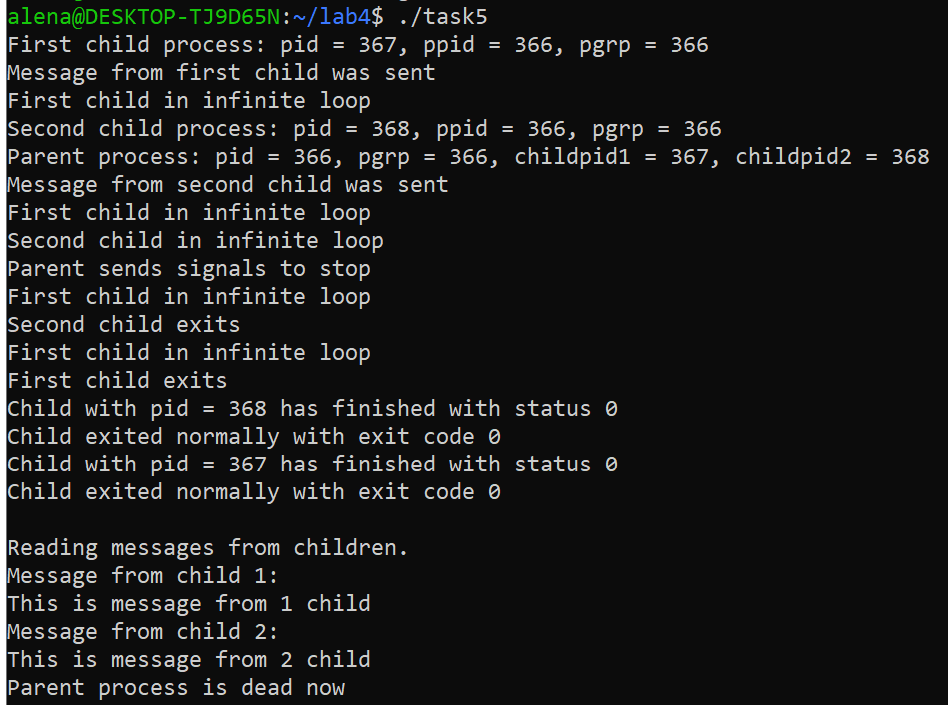
\includegraphics[width=\linewidth]{img/task05.png}
	\caption{Демонстрация работы программы (задание №5).}

	\label{fig:task05}

\end{figure}



\bibliographystyle{utf8gost705u}  % стилевой файл для оформления по ГОСТу

\bibliography{51-biblio}          % имя библиографической базы (bib-файла)


\end{document}
